\documentclass[12pt]{article}

%PACKAGES
\usepackage{graphicx}
\usepackage{epstopdf}
\usepackage[english]{babel}
\usepackage[toc,page]{appendix}
\usepackage{listings}
\usepackage{caption}
\usepackage{epsfig}
\usepackage{amsmath} % Required for some math elements 

\usepackage{hyperref}
\usepackage[left=3cm,top=3cm,right=3cm,nohead,nofoot]{geometry}
\usepackage{braket}
\usepackage{datenumber}
\usepackage{placeins}


%COMMANDS

\begin{document}

\begin{center}
\begin{figure}
\centering%
\epsfig{file=general/logo-andes.jpg,scale=0.75}%
\end{figure}
\vspace{3 cm}
\FloatBarrier
\Huge
Laniakea in a Cosmological Context\\
\vspace{3 mm}
or\\
\vspace{3 mm}
Detection of galaxy superclusters in simulated cosmological structures\\  
\vspace{1 cm}
\vspace{3mm}
\Large Sergio Daniel Hern\'{a}ndez Charpak\\

\large
200922618\\
\vspace{1 cm}
\vspace{2mm}
\Large
Advisor: Jaime E. Forero-Romero\\

\normalsize
\vspace{2mm}
\vspace{1 cm}
\today \\
\vspace{1 cm}
\small 
Universidad de los Andes\\
Facultad de Ciencias, Departamento de F\'{i}sica\\
Bogot\'{a}, Colombia\\
\end{center}


\normalsize
\newpage
\section{Acknowledgements}

I would like to thank my advisor, Jaime E. Forero-Romero, for his guidance
 during this process and of course my family,
  Nathalie, Jose Tiberio, Yv\'{a}n David,
  Gabriel Luis, Nico, Dani and all the others for
   their great patience and always good advices. I
    also acknowledge the University of Los Andes
     for its mayor financial support during my
      studies. Finally I couldn't have finish this
       work without the support of Andr\'{e}s,
        Nicol\'{a}s, Jorge and all the special
         friends I am lucky to have. Georges would
          be very happy.


\newpage
\section{Abstract}
Recently Tully et al. (2014)
 \cite{tully_laniakea_2014} used local cosmic flow
 information to define our local supercluster,
  Laniakea. 
In this work we present a study on large
 cosmological N-body
simulations aimed at establishing the significance
 of Laniakea in a
cosmological context.
We explore different algorithms to define
 superclusters from the dark
matter velocity field in the simulation. 
We summarize the properties of the supercluster
 population by their
abundance at a given total mass and its shape
 distributions.
We find that superclusters similar in size and
 structure to Laniakea are
relatively uncommon on a broader cosmological
 context.
We finalize by discussing the possible sources of
 systematics (both in
our methods and in observations) leading to this
 discrepancy.
%TODO make sure it is what it is
\newpage
\tableofcontents
\newpage

\section{Introduction}
The Universe, at large scales, has a filamentary
 scructure. Large voids regions and galaxy
  superclusters are part of it. These structures can
   be identified visually. However, there are
    different algorithms to identify them based on
     physical criteria \cite{gott_iii_map_2005}.    
\\

Due to gravitational attraction, velocity and
 density are related. It is possible to relate
  velocity fields with density fields. A proposal to
   find galaxy superclusters is to analyze the
    velocity field of galaxy. Matter tend to flow to
     the most dense region. In this way, spacial
      regions where the galaxy flow is convergent
       represent galaxy superclusters.\\
\\
Recently a team build a galaxy velocities flow map
 of the local group in a scale of hundreds of light
  years \cite{tully_cosmicflows-2_2013}. In this map
   converging points were found and this team
    identified Laniakea, the galaxy supercluster
     which includes our galaxy, the milky way
      \cite{tully_laniakea_2014}. These observations
       are difficult to make for several reasons we
        will describe briefly. As a result of these
         difficulties, there is not a statistical
          quantity of galaxy superclusters obtained
           from the observational approach. 
\\   

We propose to develop a method to detect a
 statistical significant number of galaxy
supercluster in cosmological simulations. 
With this we aim to quantify if Laniakea can be
 considered as an atypical structure in
the Universe. 
\\

\section{Background}
\subsection{Cosmic flows and peculiar velocities}
%Describe in detail the Laniakea work and the Methods used

%TODO Paragraph about the peculiar velocity.
%TODO What is the peculiar velocity in an expanding universe?

The peculiar velocity refers to the velocity relative to a rest frame. \\

%TODO Paragraph about how do you find it observationally.
In the case of the Cosmicflows-2 map, the rest frame is the earth. \\




%TODO Paragraph about the Wiener filterning method
%TODO Explain how the fieltering worked
%Reference \cite{zaroubi_wiener_1995}
A Wiener filtering method was apply to obtained a better Signal/Noise proportion and separate the peculiar velocities from the cosmic expansion.\\





\subsection{Boundaries of Laniakea - The V-Web Algorithm}
\label{sec:v_web}
The contour of the region were reconstructed with
 the V-web Algorithm. 
%TODO V-Web
%Reference \cite{hoffman_kinematic_2012}
This algorithm is deeply
  connected to the velocities as its core is the
   shear velocity tensor.\\

%TODO Explain how the V-Web algorithm worked. 





\subsection{Fractional Anisotropy and Overdensity}
\label{sec:FA_trace}
%TODO FA and Trace of the Tensor
%\cite{bustamante_tensor_2015}
%\cite{libeskind_velocity_2013}
\subsection{The Current Model: Cosmological Parameters}
\label{cosmo_constants}
%TODO Explain the cosmological Parameters
\section{Methods}
\begin{par}
Volker Springel's N-Body simulation software,
 Gadget-2 \cite{springel_gadget_2_2005}, is
  currently state-of-the-art in the field of
   cosmological simulations and is widely used in
    the scientific community. One example of use of
     Gadget is the Millennium Run
      \cite{springel_simulations_2005}, which has
       brought our understanding of our current
        model forward. We describe our numerical
         experiments in the section \ref{sec:sims}.
\end{par}
\\
\begin{par}
We devised different approaches for the detection of
 galaxy superclusters in the simulation data. One
  approach is based on the speed and is described in
   appendix \ref{App:App_Speed}. We describe our
    main approach in section \ref{sec:approaches}.
     It is based on the analysis of the 
    %TODO verify this
    eigenvalues of the local velocity shear tensor
     in the V-Web scheme. We use the Fractional
      Anisotropy and the trace of the shear tensor
       described in section \ref{sec:FA_trace}. 
\end{par}
\\
\begin{par}
We developed code in C and Python to treat the
 simulation data. The code is made available for the
  public in Github
   \url{https://github.com/sercharpak/Monografia/}
\end{par}


\subsection{Simulations}\label{sec:sims}
\begin{par}
We used the N-Body simulation software Gadget-2
 \cite{springel_gadget_2_2005}
widely used in the scientific community to
 generate different cubic boxes of dark matter
  particles
  (DM). The simulations ran on the HPC cluster at
   UNIANDES.
  The main properties (boxsize, number of
   particles, number of CPUs used and time of the
    simulation) are described in table
     \ref{tab:sims}. \\
\end{par}
\begin{itemize}
\item Numerical Experiments
\end{itemize}
\begin{par}
We are looking for structures of the same order of
 magnitude of Laniakea. Laniakea is, approximatively, a
  sphere of radius 80 Mpc/h. Our simulations need to be
   of at least the same order of magnitude. Next, we
    need to have a sufficient number of DM particles to
     be able to perform the Cloud in Cells described in
      section \ref{sec:approaches}. Finally we want
       these simulations to run in a reasonable time. 
       In table \ref{tab:sims}, we describe the 3
        simulations we ran. We first ran the Medium
         simulation, of dimension 500 Mpc/h and $512^3$
          DM particles, as a first approach to this
           problem. To perform the CIC correctly we
            needed a more dense simulation. The result
             is the Small (Dense) simulation, of
              dimension 250 Mpc/h and the same $512^3$
               DM particles. Finally we ran a longer
                Medium (Dense), of dimension 500 Mpc/h
                 and  $1024^3$ DM particles. This last
                  simulation took several days to
                   complete (80 hours). A bigger
                    simulation would take several weeks
                     and is to be performed in a future
                      work.
\end{par}
\begin{table}[ht]
    \centering
    \begin{tabular}{|c|c|c|c|c|}
        Name & Boxsize [Mpc/h] & DM particles & \# CPU & Time [hours] \\
        Medium & 500 & $512^{3}$ & 48 & ~ 10 \\
        Small (Dense) & 250 & $512^{3}$ & 48 & ~ 6  \\
        Medium (Dense) & 500 & $1024^{3}$ & 48 & ~ 80\\
    \end{tabular}
    \caption{Different Gadget-2 Simulations. We named them to easily refer to each one of them}
    \label{tab:sims}
\end{table}
\FloatBarrier

By DM particle we mean a particle which only
 interacts through gravity
interaction. In the simulation each particle
 represents a galaxy. The DM particles are
placed in a 3D grid layout first and then are
 perturbed following a Poisson distribution
before the simulation start, during the initial
 conditions generation. Once the simulation starts, the particles interact only with gravity\\

%TODO this may be could be relocated in the %background section
The initial conditions were generated with Volker
 Springel's N-Genic software. For the initial
  conditions we specify the cosmological constants
   described in section \ref{sec:cosmo_constants}. They
    are described in table \ref{tab:consts}\\.
   
  
 \begin{table}[ht]
    \centering
    \begin{tabular}{|c|c|c|c|}
        $\Omega_0$ & $\Omega_{\Lambda}$ & $\Omega$ & H \\
        0.3 &  0.7 & 0 & 0.7 \\
    \end{tabular}
    \caption{Cosmological Constants in the Gadget-2 Simulations}
    \label{tab:consts}
\end{table}
\FloatBarrier
%TODO Specify the units
$\Omega_0$  corresponds to the Cosmological matter density parameter in units of the critical density at
red shift z = 0. $\Omega_{\Lambda}$ is the cosmological
 vacuum energy density (cosmological constant) in
  units of the critical density at red shift z = 0. 
%Relevant only for comoving integration. 
For a geometrically flat universe, as ours, one has $\Omega_0$ + $\Omega_{\Lambda}$ = 1.
 $\Omega$ is the baryon density in units
  of the critical density at red shift z = 0. In our case it
   is not relevant. Finally, H denotes the Hubble
    constant at red shift z=0 in  units of 100 $km$ $s^{-1}$
     $Mpc^{-1}$. It will be relevant in the
      discussions, section \ref{sec:discussions}.
%TODO make a reference to the discussion with the
% Chon paper where the Hubble constant is related
% to a gravitationaly bounded structure.
%TODO Explain the constants

We then use different algorithms to identify the
 superclusters within the simulation.\\

\subsection{Approaches} \label{sec:approaches}
%Opening the section
\begin{par}
In a first approach we analyse the distribution of
 the magnitude of the velocity in the different
  simulations. We work with all the particles and
   points given by the simulation. As our final
    results are not based in this naive approach
     we leave it as an appendix here. It is
      explained in further detail in Appendix
       \ref{App:App_Speed}.\\
\end{par}

\begin{par}
For our second approach (main one), we will use the
 following concepts: Cloud In Cell (CIC) method, the V-
 Web scheme (as described in section \ref{sec:v_web}),
  the Fractional Anisotropy (FA) (as described in
   section \ref{sec:FA_trace}), the trace of the
    velocity shear tensor $tr\left(\sum_{\alpha
     \beta}\right)$ (as described in section
      \ref{sec:FA_trace}) and the algorithms described
       in section \ref{sec:algorithms}.\\
\end{par}


\begin{itemize}
\item The Cloud In Cell (CIC) method
\end{itemize}
\begin{par}
%TODO Describe the CIC method
The Cloud In Cell (CIC) method is a derivation of the
 Particle in Cell (PIC) method, a Particle Mesh (PM)
  method, first introduced by Francis Harlow in the
   1950's in the field of computational fluid dynamics
    \cite{harlow1964particle}. CIC is very popular
     among the scientific community
      \cite{grigoryev_numerical_2002}. We form, in our
       case, a $N^3$ grid. This grid is superpose with
        the cubic
      box resulting from the simulation. We then form
       particle clouds (cubes in our case) around each
        particle. For each particle cloud, each cell
         where the particle cloud superposes is
          assigned a weighted part of the physical
           quantity we look to mesh proportional to the
            superposed volume (in 2-D, superposed
             area). We perform this CIC
            for the density field and the velocity
             field. In figure \ref{fg:cic_explain} a
              graphical explanation is provided for the
               2-D case.  \\
\end{par}

\begin{figure}[ht]
\begin{center}
\includegraphics[width=0.6\textwidth]{general/CIC_Explain_bigger} % Include the image placeholder.png
\caption{Explanation of the Cloud In Cell Method (CIC)}
\label{fg:cic_explain}
\end{center}
\end{figure}
\FloatBarrier

\begin{itemize}
\item The V-Web scheme
\end{itemize}
\begin{par}
%TODO Describe very briefly the V-Web
We described the V-Web scheme in section \ref{sec:v_web}.\\ %TODO write a summary of the V-WEB
\end{par}

\begin{itemize}
\item The Fractional Anisotropy and the trace of $\sum_{\alpha \beta}$
\end{itemize}
\begin{par}
%TODO Describe very briefly our use of FA and $\sum_{\alpha \beta}$
As we saw in section \ref{sec:FA_trace} the FA and the trace of $\sum_{\alpha \beta}$ carry valuable information.
The FA %TODO what iformation carries the FA

The trace of $\sum_{\alpha \beta}$\\  %TODO what iformation carries the $\sum_{\alpha \beta}$
\end{par}


\begin{par}
In summary, our approach follows the steps:
\end{par}

\begin{enumerate}
\item Calculate the density field using CIC on the simulation data.
\item At the same time we calculate the velocity field using CIC on the simulation data.
\item Using finite differences we form the velocity shear tensor $\sum_{\alpha \beta}$.
\item We diagonalize it and find its eigenvalues $\lambda_i$ and eigenvectors $\hat{u}_i$
\item We form the FA grid as described in section \ref{sec:FA_trace} 
\item We form the trace of $\sum_{\alpha \beta}$ grid.
\item We apply the algorithms described in section \ref{sec:algorithms} to find the superclusters
\item We extract the properties (volume, shape, mass) from the superclusters
\item We compare the superclusters to Laniakea
\end{enumerate}




%Closing the section
\begin{par}
Our approach is hence very close with the approach
 used to define Laniakea
  \cite{tully_laniakea_2014} which is important to
   validate our later comparison of Laniakea with
    our detected structures.
\end{par}

\subsection{Algorithms}\label{sec:algorithms}

Our main algorithm is a region growing algorithm
 as described by Gonzalez
  \cite{gonzalez_digital_2008} mainly used in
   image segmentation. We now proceed to describe
    it generally.
\subsubsection{Region Growing Algorithm: Basic Description}

\begin{par}
The region growing algorithm is used to identify different regions in a image. The aim is to identify regions which share common properties. First we identify points, as few as possible, which we know for sure are contained in these regions. These points are the seeds of our regions. We then define a certain growth predicate, if the neighbours of a seed validate this predicate they are considered as members of the group. These new members are then treated as seeds and ask their own neighbours if they validate the predicate. This goes on until all the points have been evaluated or until a limit defined by the user is reached.
\end{par}

\begin{par}
We can write in a more formal way:
\end{par}

\begin{par}
$f(x,y,z)$ denotes the input data. $S(x,y,z)$ denotes a seed array, with
value 1 where the particle can be define as a seed and 0 where not. $S(x,y,z)$ is the
same size of $f(x,y,z)$. $Q$ denotes a predicate which is to be apply to the
input data and determines if the region which
 starts at the seeds grows or
not. 
\end{par}

\begin{enumerate}
	\item We search for seeds from $f(x,y,z)$ based in a criterion
	\item For each detected seed, we change the values of $S(x,y,z)$ to 1 at the seed's coordinates.
	\item For each detected seed, we iterate its neighbors if they validate the predicate $Q$.
    \item If the particle $c$ at $x_c, y_c, z_c$ satisfies $Q$, it is marked as part of the region, $S(x_c, y_c, z_c) = 1$
    \item Apply the algorithm to $c$, and so on
     (Recursion).
\end{enumerate}

\begin{par}
The algorithm is based on a connectivity concept (definition of
neighbours). Here we are working on a 4-connectivity. 4
connectivity means that no diagonal particles are considered as
neighbours. The following matrix shows this principle in a 2
dimensional case. Only the elements labelled as 1 are considered as
neighbours of the center $C$.
\end{par}

\[ 
\begin{bmatrix} 
    0 & 1 & 0 \\
    1 & C & 1 \\
    0 & 1 & 0\\
\end{bmatrix} 
\]

\begin{par}
So, if a particle is in coordinates $(x,y,z)$ its neighbours are
$(x-1,y,z)$, $(x+1,y,z)$, $(x,y-1,z)$, $(x,y+1,z)$, $(x,y,z-1)$
and $(x,y,z+1)$.
\end{par}

\begin{par}
Another widely used connectivity is the 8-connectivity. As it is
intuitive, in 8-connectivity, the diagonal particles are also
considered as neighbours. We decided to use 4-connectivity to
simplify our own implementation.
\end{par}




\subsubsection{Region Growing Algorithm with the FA and the trace of the velocity shear tensor}\label{sec:own_impl_descr}
Our implementation is based in the FA and the trace of the velocity shear tensor $tr\left(\sum_{\alpha \beta}\right)$. It is uses 4-connectivity as described before.

\begin{itemize}
    \item Seeds
\begin{par}
We are looking for overdense structures. Therefore we will look
for particles with $tr\sum_{\alpha \beta} \geq 1.0$.  We also want to analyse how
the FA fits. We know that the centres of our structures should be
fairly isotropic so we will explore seeds with FA lesser than a
threshold. We will perform several runs of the algorithm, so we
can explore the different criterion for the choice of the seeds.
These can be seen in table \ref{tab:seeds_FA_Trace}. 
\end{par}
 \begin{table}[ht]
    \centering
    \begin{tabular}{|c|c|c|c|}
        $FA_{seed}$ & $tr\left(\sum_{\alpha \beta}\right)_{seed}$ \\
        0.5 &  1.0 \\
        0.6 &  1.0 \\
        0.7 &  1.0 \\
        0.8 &  1.0 \\
        0.9 &  1.0 \\
    \end{tabular}
    \caption{Different values of the FA and $tr\left(\sum_{\alpha \beta}\right)$ for the choice of the seeds}
    \label{tab:seeds_FA_Trace}
\end{table}
\FloatBarrier

\item Labelling the regions
\begin{par}
We label groups as a function of its respective
 seed to extract properties (volume, shape, mass)
  for each one of them.
\end{par}

\item Predicate $Q$

\begin{par}
We define, as we did for the
choice of the seeds, thresholds for the FA and for $tr\left(\sum_{\alpha \beta}\right)$. If
the neighbour cell validates these thresholds, and hasn't been
labelled yet, it is labelled as the group of the seed particle. So
in other words: \\

\begin{center}
$Q: \left( FA (x,y,z) \leq Thresh_{FA} \right)$ AND
$\left( \delta (x,y,z) \geq Thresh_{tr\left(\sum_{\alpha \beta}\right)} \right)$ 
\end{center}
As we are looking for overdense regions (no voids) we define the
threshold for $tr\left(\sum_{\alpha \beta}\right)$ as 0.0. As we are exploring the different
values for the FA. each run will follow a row of the table \ref{tab:search_FA_Trace}.
\end{par}

\begin{table}[ht]
    \centering
    \begin{tabular}{|c|c|c|c|}
        $FA_{growth}$ & $tr\left(\sum_{\alpha \beta}\right)_{growth}$ \\
        0.5 &  0.0 \\
        0.6 &  0.0 \\
        0.7 &  0.0 \\
        0.8 &  0.0 \\
        0.9 &  0.0 \\
    \end{tabular}
    \caption{Different values of the FA and $tr\left(\sum_{\alpha \beta}\right)$ for the growth of the regions}
    \label{tab:search_FA_Trace}
\end{table}
\FloatBarrier

\end{itemize}

\begin{par}
A simplified version without the border cases
 management can be seen in appendix \ref{App:own_impl_code}. Results of this
  implementation can be seen in section
   \ref{sec:results_own_impl}.
%TODO put in appendix the simplified code
%TODO The results could also be put in the appendix
\end{par}

%\subsubsection{FoF with the FA and Overdensity}\label{sec:fof_impl_descr}
\begin{par}
Finally to find the groups we used the Friends-of-Friends (FoF) algorithm.
\end{par}
%TODO Describe the FoF and the final pipeline implementation
\begin{par}
The FoF algorithm looks at the distances between points in a given
set. If the distance between a point $a$ and a point $b$ is less
than a predefined threshold, $a$ and $b$ now form a region. For a
region to be created by the FoF algorithm it also needs to have a
predefined minimum number of members. 
\end{par}

\begin{par}
We choose as set of points all the
particles which validate the predicate $Q$ (following table
\ref{tab:search_FA_Trace}, as maximum distance the distance
between one particle and its neighbours as described by
4-connectivity. And we use the FoF algorithm to form the groups. 
\end{par}
\begin{par}
We search for the seeds following table \ref{tab:seeds_FA_Trace}
and obtain a list of the seeds. We then proceed to validate which
of the groups obtained by the FoF is a valid group. To be
considered as a valid group, it needs to contain at least one seed
particle. This procedure allow us to take care of the case where
two seeds form two groups which eventually get together. Now we
can make sure these groups are merged into one and there is no
need to search for this case individually.
\end{par}


\section{Results}

\subsection{General visualizations (FA, $\delta$) of the Simulations}

\subsubsection{FA, Fractal Anisotropy}
Using our small and dense simulation described in table \ref{tab:sims}, after the CIC (in a $256^{3}$ grid) and V-Web have been applied, we can form the FA and visualize its histogram (Figure \ref{fg:hist_FA}) and a 2-D cut (Figure \ref{fg:cut_FA}).
%Histogram and cut
\begin{figure}[ht]
\centering
\begin{minipage}{.5\textwidth}
  \centering
  \includegraphics[width=0.8\textwidth]{simulation/FA_hist_sim.png}
  \caption{FA Histogram of the Small and Dense simulation}
\label{fg:hist_FA}
\end{minipage}%
\begin{minipage}{.5\textwidth}
  \centering
  \includegraphics[width=0.95\textwidth]{simulation/FA_cut_i_10.png}
  \caption{A cut of the FA in the x axis}
\label{fg:cut_FA}
\end{minipage}
\end{figure}
\FloatBarrier

%TODO Correct the following statement.
\begin{par}
As we saw in section \ref{sec:FA_trace}, you would
 expect to have few highly isotropic particles.
  The distribution \ref{fg:hist_FA} we obtained
   agrees with it.\\
Observing a 2-D cut of the FA \ref{fg:cut_FA} we
 observe the filamentary structures we would
  expect of the Cosmic Web. This cut is very
   similar to the ones presented by  Bustamante et
   al.  \cite{bustamante_tensor_2015} in their
    work. This is a good indicator that our
     simulation, CIC procedure V-Web application
      and FA forming were correctly executed.
       Bustamante et. al  explain that void
        regions should have a FA < 0.95. We expect
         the similar FA values for superclusters
          and will make use of the Overdensity
           $\delta$ to discriminate the    
            regions and make sure we do not find
             voids.

\end{par}


\subsubsection{$\delta$, Overdensity}
As we did for the FA, we visualize the
 distribution (Figure \ref{fg:hist_Trace}) and a
  2-D cut (Figure \ref{fg:cut_Trace})of $\delta$
   for the small and dense simulation of table
    \ref{tab:sims}.

%Histogram and cut
\begin{figure}[ht]
\centering
\begin{minipage}{.5\textwidth}
  \centering
  \includegraphics[width=0.8\textwidth]{simulation/Trace_hist_sim.png} % Include the image placeholder.png
\caption{$\delta$ Histogram of the Small and Dense simulation}
\label{fg:hist_Trace}
\end{minipage}%
\begin{minipage}{.5\textwidth}
  \centering
  \includegraphics[width=0.95\textwidth]{simulation/Trace_cut_i_10.png}
  \caption{A cut of the $\delta$ in the x axis}
\label{fg:cut_Trace}
\end{minipage}
\end{figure}
\FloatBarrier

\begin{par}
The overdensity $\delta$ distribution is symmetric
 around 0.0. As we are searching for overdense
  structures (superclusters) we can then diminish
   our search space to half of it only by
    selecting the points with $\delta \geq 0.0$. \\
Observing a 2D cut of the overdensity as shown in
 figure \ref{fg:cut_Trace} also gives a good idea
  of good idea of the Cosmic Web as we can easily
   recognize filaments (highly underdense, $\delta
    \leq 1.0$) and highly overdense regions
     ($\delta \geq 1.0$) which are our candidates
      for seeds of supercluster structures.
\end{par}



\subsection{Region Growing Algorithm with the FA and Overdensity} \label{sec:results_own_impl}
%The first results I got
%TODO this section could be ommited and just show the last results (the next section)
\begin{par}
Using our small and dense simulation described in
 table \ref{tab:sims}, after the CIC (in a
  256x256x256 grid) and V-Web have been applied,
   we ran the implementation described in section
    \ref{sec:own_impl_descr} for some of the
     values described in tables
      \ref{tab:seeds_FA_Trace} and
       \ref{tab:search_FA_Trace}. 
\end{par}

\begin{figure}[ht]
\begin{center}
\includegraphics[width=0.7\textwidth]{groups/firstimplementation/regions_3D_129.png} % Include the image placeholder.png
\caption{Regions detected for: Seeds (FA:0.6, $\delta$: 1.0) and Growth (FA:0.8, $\delta$: 0.0) }
\label{fg:first_3D_all}
\end{center}
\end{figure}
\FloatBarrier

\begin{figure}[ht]
\centering
\begin{minipage}{.5\textwidth}
  \centering
  \includegraphics[width=0.8\textwidth]{groups/firstimplementation/largest_vol_24_seeds_129.png} % Include the image placeholder.png
\end{minipage}%
\begin{minipage}{.5\textwidth}
  \centering
  \includegraphics[width=0.8\textwidth]{groups/firstimplementation/largest_vol_24_seeds_129_scale.png}
  \end{minipage}
\caption{Largest volume detected for: Seeds (FA:0.6, $\delta$: 1.0) and Growth (FA:0.8, $\delta$: 0.0). The region is on the left and can be seen at scale with the simulation on the right.}
\label{fg:first_3D_largest}
\end{figure}
\FloatBarrier

\subsection{Region Growing Algorithm and FoF with the FA and Overdensity}
%The real results I got

\begin{par}
For the results of the small and dense simulation \ref{tab:sims} we applied all the combinations for thresholds in tables \ref{tab:seeds_FA_Trace} (seeds)  and \ref{tab:search_FA_Trace} (growth). 
\end{par}

\subsubsection{Influence of the FA in the seeds}

\begin{figure}[ht]
\centering
\begin{minipage}{.45\textwidth}
  \centering
  \includegraphics[width=0.9\textwidth]{groups/3d/seeds_FA_5/regions_nonoise_seeds_FA_05_Trace_10_search_FA_09_Trace_00_.png}
\end{minipage}%
\begin{minipage}{.45\textwidth}
  \centering
  \includegraphics[width=0.9\textwidth]{groups/3d/seeds_FA_6/regions_nonoise_seeds_FA_06_Trace_10_search_FA_09_Trace_00_.png}
\end{minipage}
\begin{minipage}{.45\textwidth}
  \centering
  \includegraphics[width=0.9\textwidth]{groups/3d/seeds_FA_7/regions_nonoise_seeds_FA_07_Trace_10_search_FA_09_Trace_00_.png}
\end{minipage}
\begin{minipage}{.45\textwidth}
  \centering
  \includegraphics[width=0.9\textwidth]{groups/3d/seeds_FA_8/regions_nonoise_seeds_FA_08_Trace_10_search_FA_09_Trace_00_.png}
\end{minipage}
\caption{Efect of augmenting the FA threshold in the seed chosing. From upper left to down right the FA for the seeds are: 0.5, 0.6, 0.7 and 0.8. The growth FA is 0.9 and $\delta$ is 0.0. The $\delta$ for the seeds is 1.0.} \label{fg:3D_FA_seeds}
\end{figure}
\FloatBarrier

\subsubsection{Influence of the FA in the growth}
\begin{figure}[ht]
\centering
\begin{minipage}{.45\textwidth}
  \centering
  \includegraphics[width=0.9\textwidth]{groups/3d/seeds_FA_6/regions_nonoise_seeds_FA_06_Trace_10_search_FA_06_Trace_00_.png}
\end{minipage}%
\begin{minipage}{.45\textwidth}
  \centering
  \includegraphics[width=0.9\textwidth]{groups/3d/seeds_FA_6/regions_nonoise_seeds_FA_06_Trace_10_search_FA_07_Trace_00_.png}
\end{minipage}
\begin{minipage}{.45\textwidth}
  \centering
  \includegraphics[width=0.9\textwidth]{groups/3d/seeds_FA_6/regions_nonoise_seeds_FA_06_Trace_10_search_FA_08_Trace_00_.png}
\end{minipage}
\begin{minipage}{.45\textwidth}
  \centering
  \includegraphics[width=0.9\textwidth]{groups/3d/seeds_FA_6/regions_nonoise_seeds_FA_06_Trace_10_search_FA_09_Trace_00_.png}
\end{minipage}
\caption{Efect of augmenting the FA threshold in the growth. From upper left to down right the FA for the growth is: 0.6, 0.7, 0.8 and 0.9. The seed FA is 0.6 and $\delta$ is 1.0. The $\delta$ for the growth is 0.0.} \label{fg:3D_FA_growth}
\end{figure}
\FloatBarrier

\begin{par}
 We can see in figure \ref{fg:3D_FA_growth} how augmenting the FA thresholds for the growth changes drastically the volumes of the regions detected. This can also be seen comparing the possible growth space volume with the volume of the largest region detected ratio (figure \ref{fg:vol_FA_growth}).
\end{par}

\begin{figure}[ht]
\centering
\begin{minipage}{.45\textwidth}
  \centering
  \includegraphics[width=0.75\textwidth]{groups/volumeplots/volumes_growth_FA05_Trace_10.png}
\end{minipage}
\begin{minipage}{.45\textwidth}
  \centering
  \includegraphics[width=0.75\textwidth]{groups/volumeplots/volumes_growth_FA06_Trace_10.png}
\end{minipage}
\begin{minipage}{.45\textwidth}
  \centering
  \includegraphics[width=0.75\textwidth]{groups/volumeplots/volumes_growth_FA07_Trace_10.png}
\end{minipage}
\begin{minipage}{.45\textwidth}
  \centering
  \includegraphics[width=0.75\textwidth]{groups/volumeplots/volumes_growth_FA08_Trace_10.png}
\end{minipage}
%  \centering
%  \includegraphics[width=0.9\textwidth]%{groups/volumeplots/volumes_growth_FA09_Trace_10.png}
%\end{minipage}
\caption{Volume of the largest structure and Volume of the growth space ratio augmenting the FA threshold in the growth. From upper left to down right the FA for the seeds is: 0.5, 0.6, 0.7 and 0.8. The growth $\delta$ is 1.0. The $\delta$ for the seed is 0.0.} \label{fg:vol_FA_growth}
\end{figure}
\FloatBarrier

\subsubsection{Volume distribution}

\subsubsection{Shape of the regions}

\subsection{Comparisons with Laniakea}

\section{Discussions}
\label{sec:discussions}

\section{Conclusions}

%TODO The Future Work section needs to be re-written
\section{Future Work}
\label{sec:future_work}




\bibliographystyle{unsrt}
%\renewcommand\refname{Referencias}
\bibliography{references}

\appendix
\section{Approach by the Speed} \label{App:App_Speed}
\subsection{Region Growing Algorithm with the Speed}

We present here a naive way to approach to the problem. 
\begin{enumerate}
	\item We calculate the magnitude of the velocity (the speed) of each particle. 
	\item We look for regions where the center has the highest speed and from it the speed decreases while the particle is further away from the center. 
    \item We define the limits of this region the regions where the speed begins to increase with the distance from the center.
\end{enumerate}

\begin{par}
We use a region growing algorithm, a simple image segmentation algorithm
used to identify different regions in a image \cite{gonzalez_digital_2008}.
\end{par}

\begin{par}
$f(x,y,z)$ denotes the input data. $S(x,y,z)$ denotes a seed array, with
value 1 where the particle can be define as a seed and 0 where not. It is the
same size of $f(x,y,z)$. $Q$ denotes a predicate which is to be apply to the
input data and determines if the region which
 starts at the seeds grows or
not. Here $Q$ denotes: "if the speed of the close
 particle is lower than the
marked one but greater than a threshold, mark that
 particle and continue."
\end{par}

\begin{enumerate}
	\item We choose seeds to begin the growth. In
	 this case we choose the particles with high
	  velocities. Here \[ |v|>  th_{high}\]
	\item We open a window of particles to look
	 for 2 close particles from the seed $s$ which
	  do not for part of $S(x,y,z)$. Here:
    \[ window = 20000\]
    \item Once we found the 2 close particles $c$ we apply the predicate $Q$. Here:
    \[ Q := |v_s| > |v_c| > |th_{low}|\]
    
    \item If the particle $c$ satisfies $Q$, it is
     marked, $S(c) = 1$
    \item Apply the algorithm to $c$, and so on
     (Recursion).
\end{enumerate}

Here we defined empirically different thresholds
 in order to observer the results. \\
First we used:  \\
$th_{low} = v_{min} + \frac{\sigma_{v}}{2} $ and
 $th_{high} = v_{max}  - \sigma_{v}$ .\\
Secondly we used: \\
$th_{low} = \vec{v} + 2  \sigma_{v} $ and $th_{high} = \vec{v}  +  8 \sigma_{v}$.\\

The first version of the algorithm was written in
 python using the module
pyGadgetReader
 \cite{thompson_pygadgetreader_2014ascl_soft11001T}
  to read the
data and transform it to NumPy arrays in Python.
 In Appendix \ref{App:App_speed_code} we attach
  the source code used.

\subsection{Results of the Speed Approach}
This approach was tested on the simulation of
 boxsize 500 Mpc/h
and $512^{3}$ dark matter particles (DM) described
 in table \ref{tab:sims}. \\

We first visualize the speed histogram in figure
 \ref{fg:hist_vel}.\\

%Speed histogram
\begin{figure}[ht]
\begin{center}
\includegraphics[width=0.9\textwidth]{graphs/hist_vel.png} % Include the image placeholder.png
\caption{Speed Histogram of the simulation}
\label{fg:hist_vel}
\end{center}
\end{figure}
\FloatBarrier

The histogram resembles a Poisson distribution. This is a consequence of the perturbations generated in the initial conditions generation. 

\begin{table}[ht]
    \centering
    \begin{tabular}{|c|c|}
        $v_{max}$ & 2023.87 \\
        $v_{min}$ & 0.34\\
        $\sigma_{v}$ & 117.75 
    \end{tabular}
    \caption{Properties of the speed distribution}
    \label{tab:vel}
\end{table}
\FloatBarrier

Our hypothesis is based on the most direct implication of gravity. The lower speed
particles will mainly be in the border regions and the higher speed particles
will be in the center regions. \\

For this we must choose a threshold for low velocities and a threshold for high velocities. 
We obtain: $th_{low} = v_{min} + \frac{\sigma_{v}}{2} = 59.2$ and $th_{high} = v_{max}  - \sigma_{v} = 1906.12 $

%Plot 3Ds
%First 3D plot, particles with speed lower than thresh_low
We first have a look at the particle distribution of particles with speed higher than the
threshold for low velocities.\\
%59.216707265
\begin{figure}[ht]
\begin{center}
\includegraphics[width=0.8\textwidth]{graphs/pos_3d_vel_menor_s_smaller.png} % Include the image placeholder.png
\caption{DM particles with $|v| < 59.2 $}
\label{fg:3d_thresh_low}
\end{center}
\end{figure}
\FloatBarrier

There seem to be some structures, but it is not clear enough. This is due to the high number of DM particles used in this simulation ($512^3$). 

%Second 3D plot, particles with speed higher than thresh_high

We produce cuts in the z-direction to visualize in 2-D the speed distribution. \\

%Plot 2D

%5 plots of the 2D. 
\begin{figure}[ht]
\centering
\begin{minipage}{.45\textwidth}
  \centering
  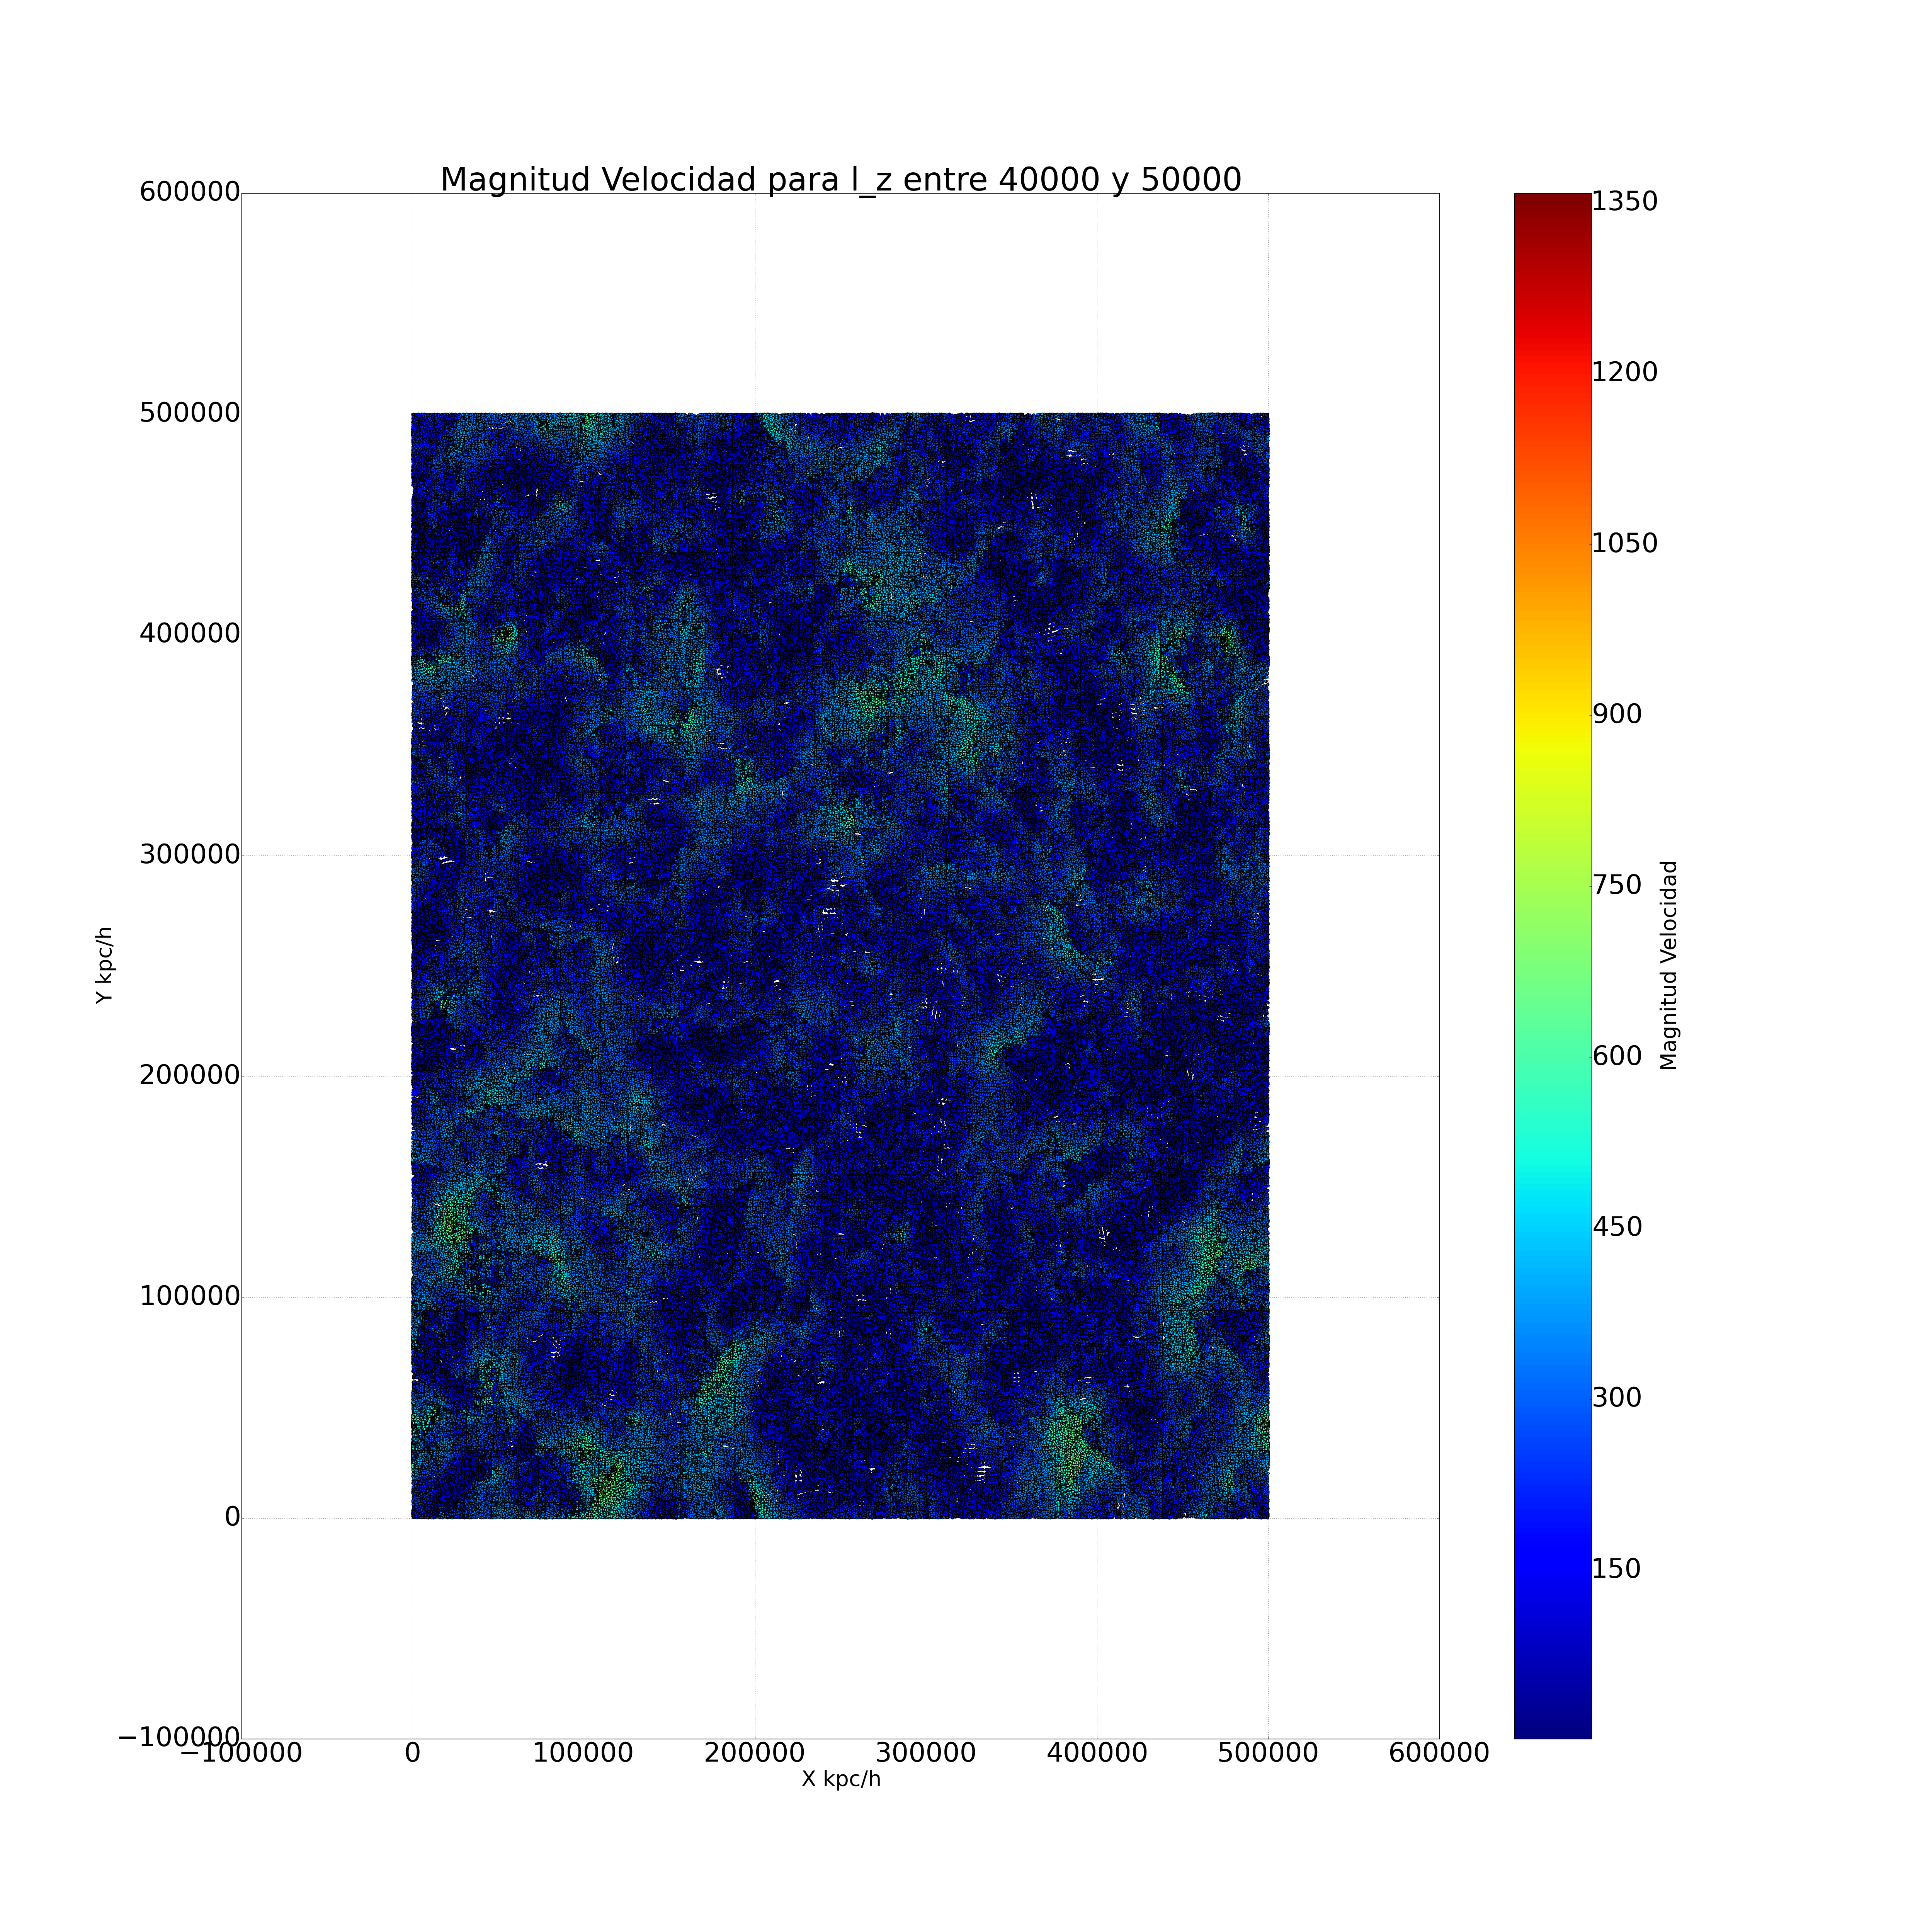
\includegraphics[width=0.9\textwidth]{graphs/scatter_magnitud_vel50000.png}
\end{minipage}%
\begin{minipage}{.45\textwidth}
  \centering
  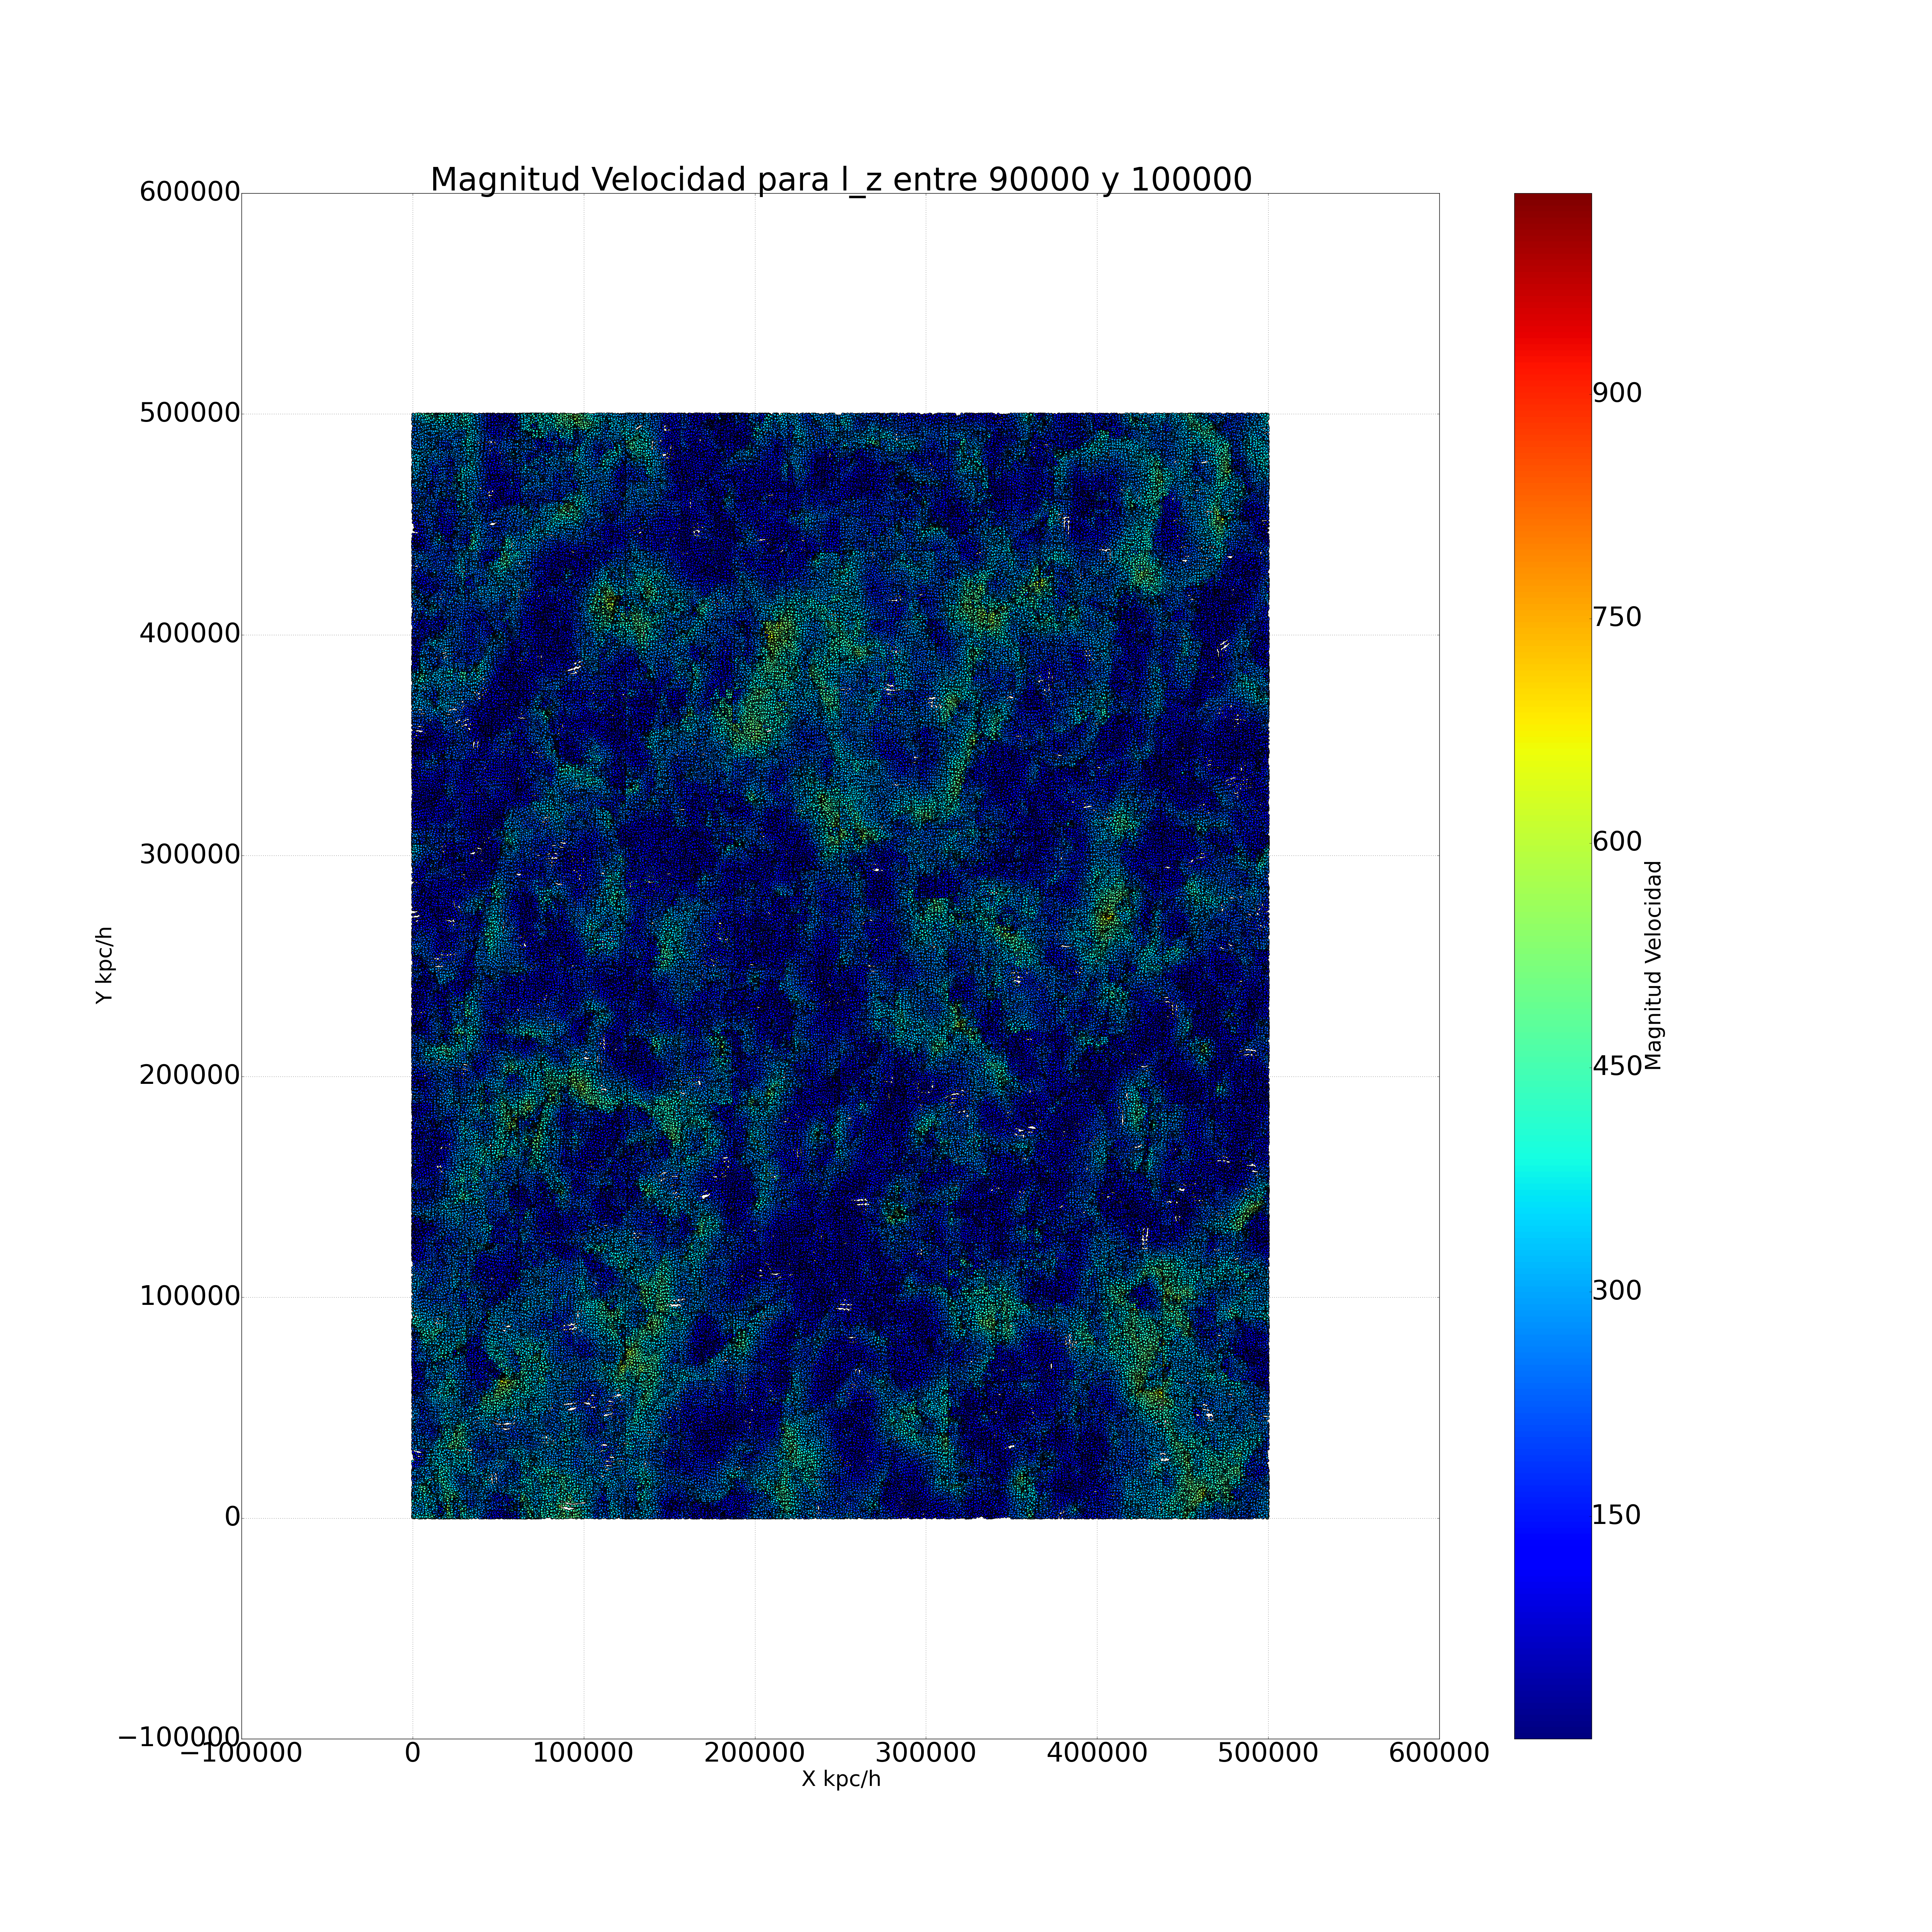
\includegraphics[width=0.9\textwidth]{graphs/scatter_magnitud_vel100000.png}
\end{minipage}
\begin{minipage}{.45\textwidth}
  \centering
  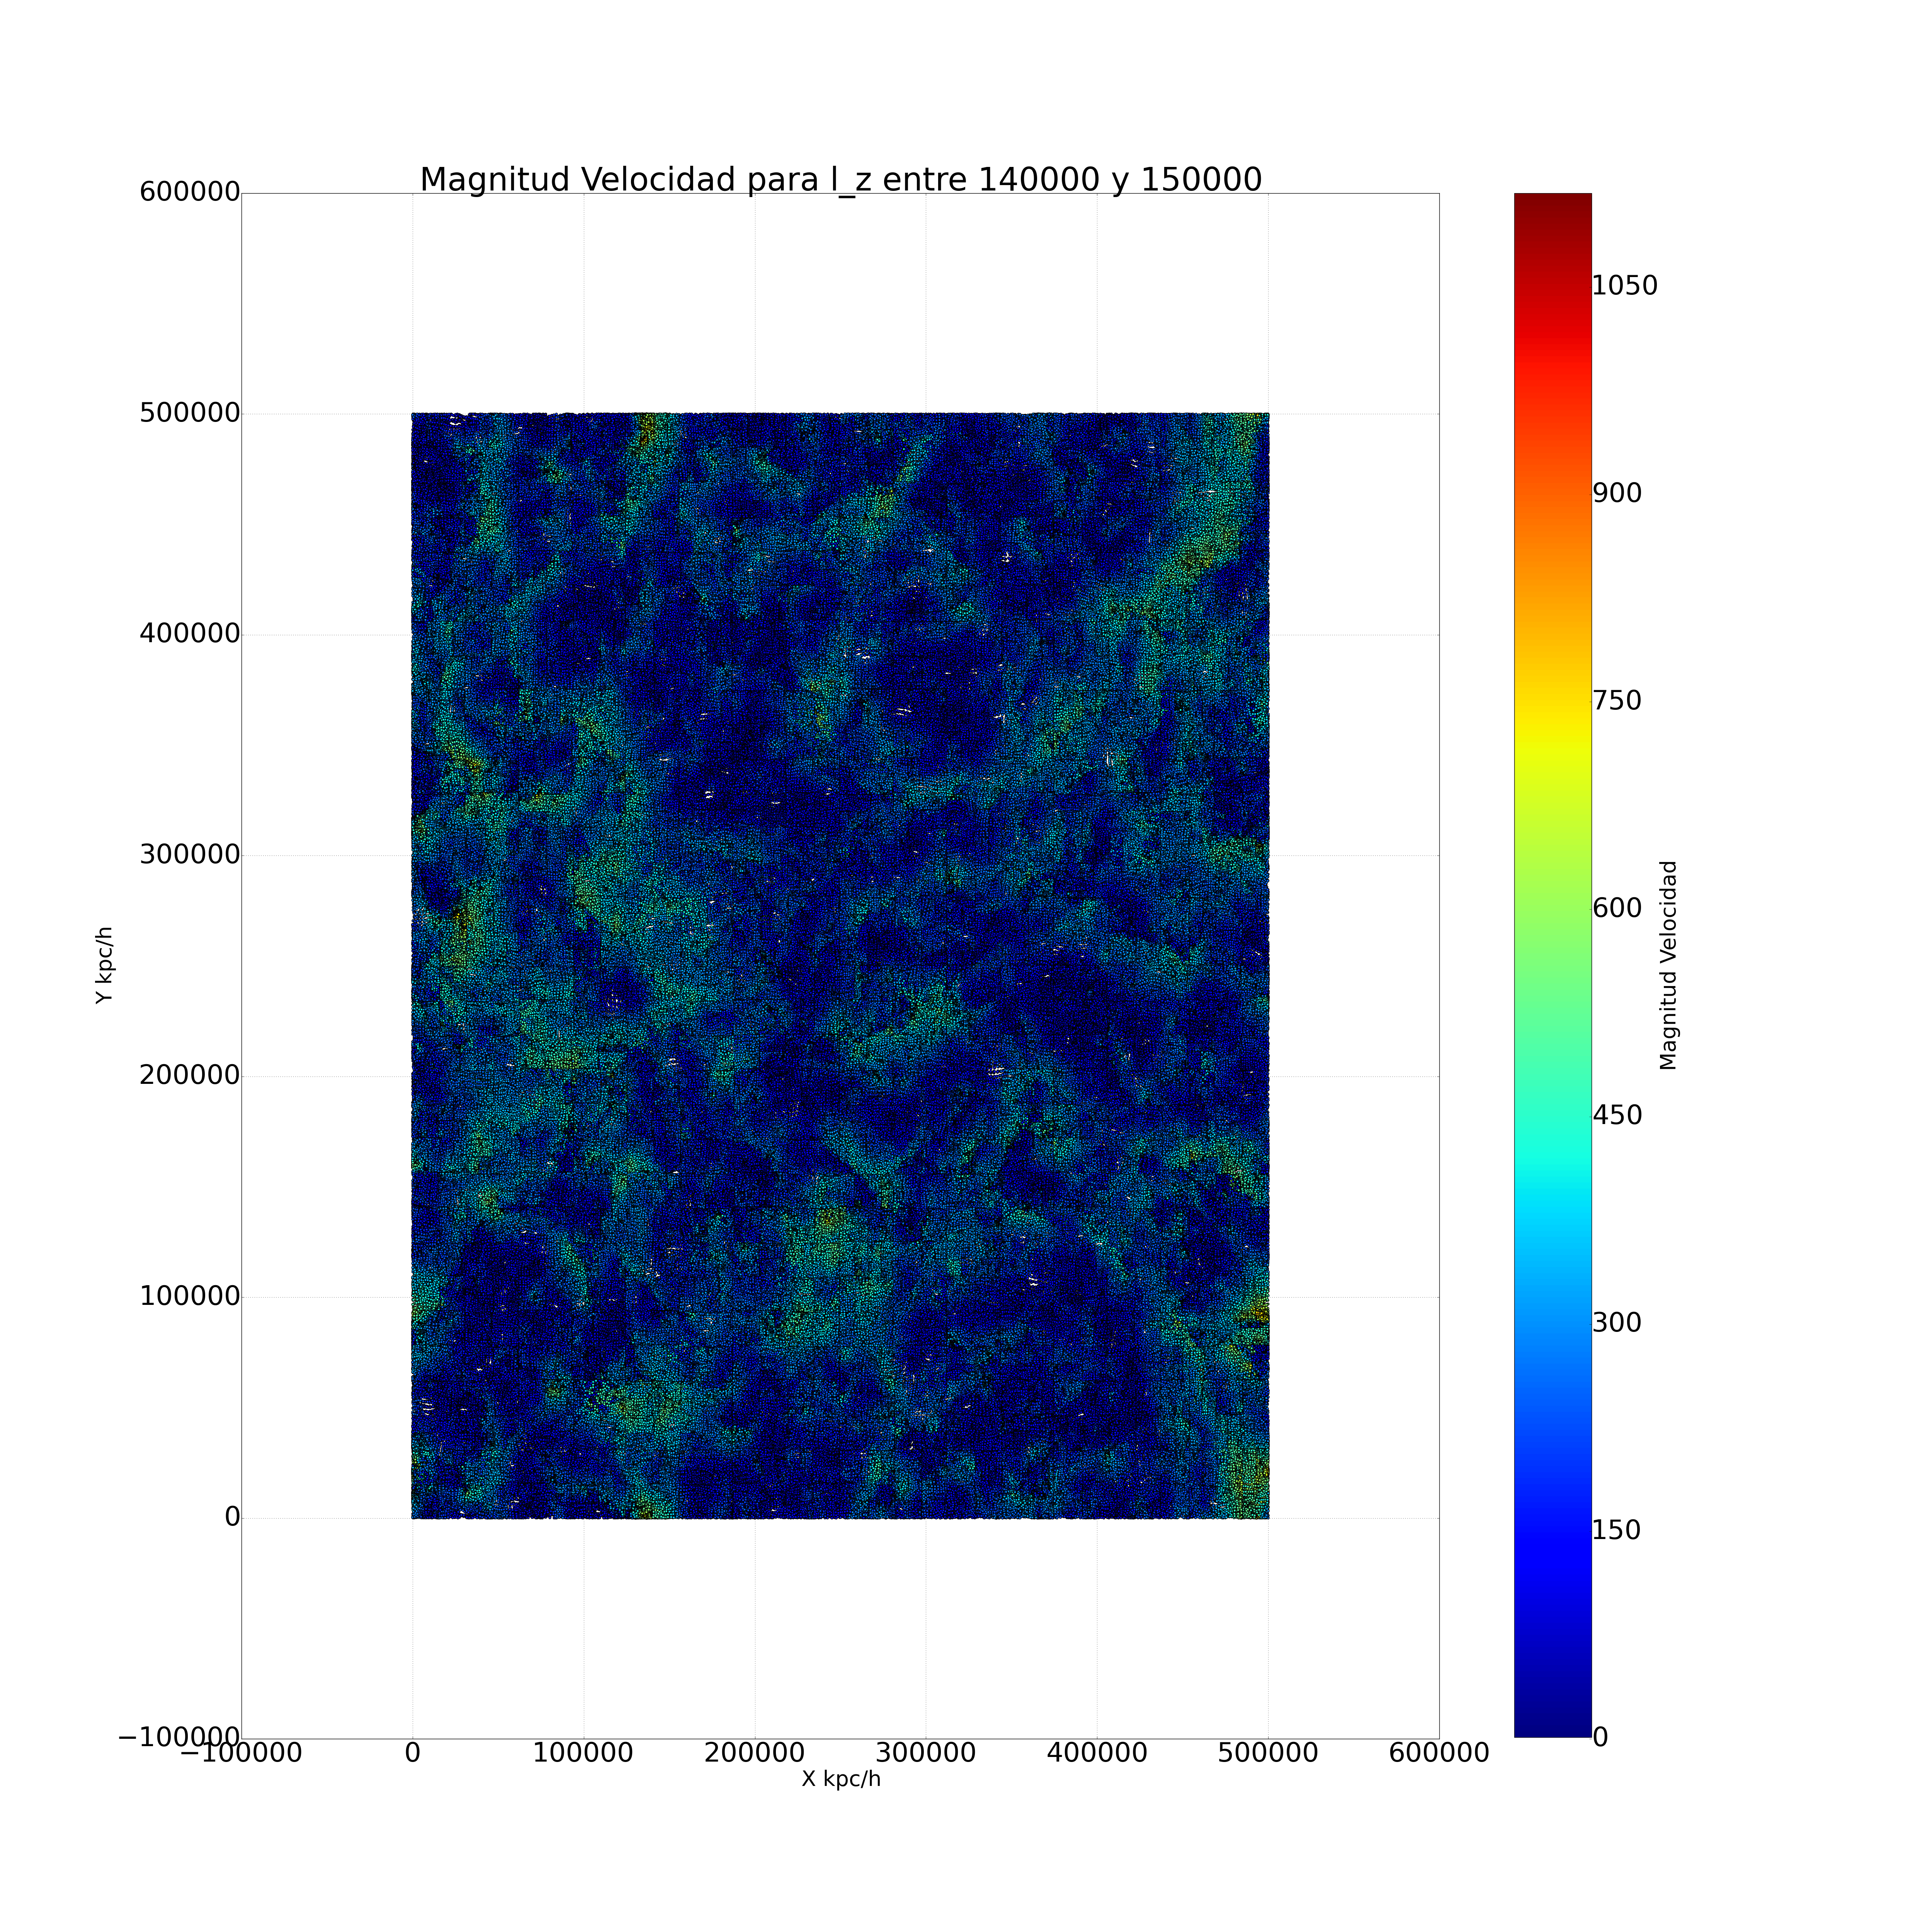
\includegraphics[width=0.9\textwidth]{graphs/scatter_magnitud_vel150000.png}
\end{minipage}
\begin{minipage}{.45\textwidth}
  \centering
  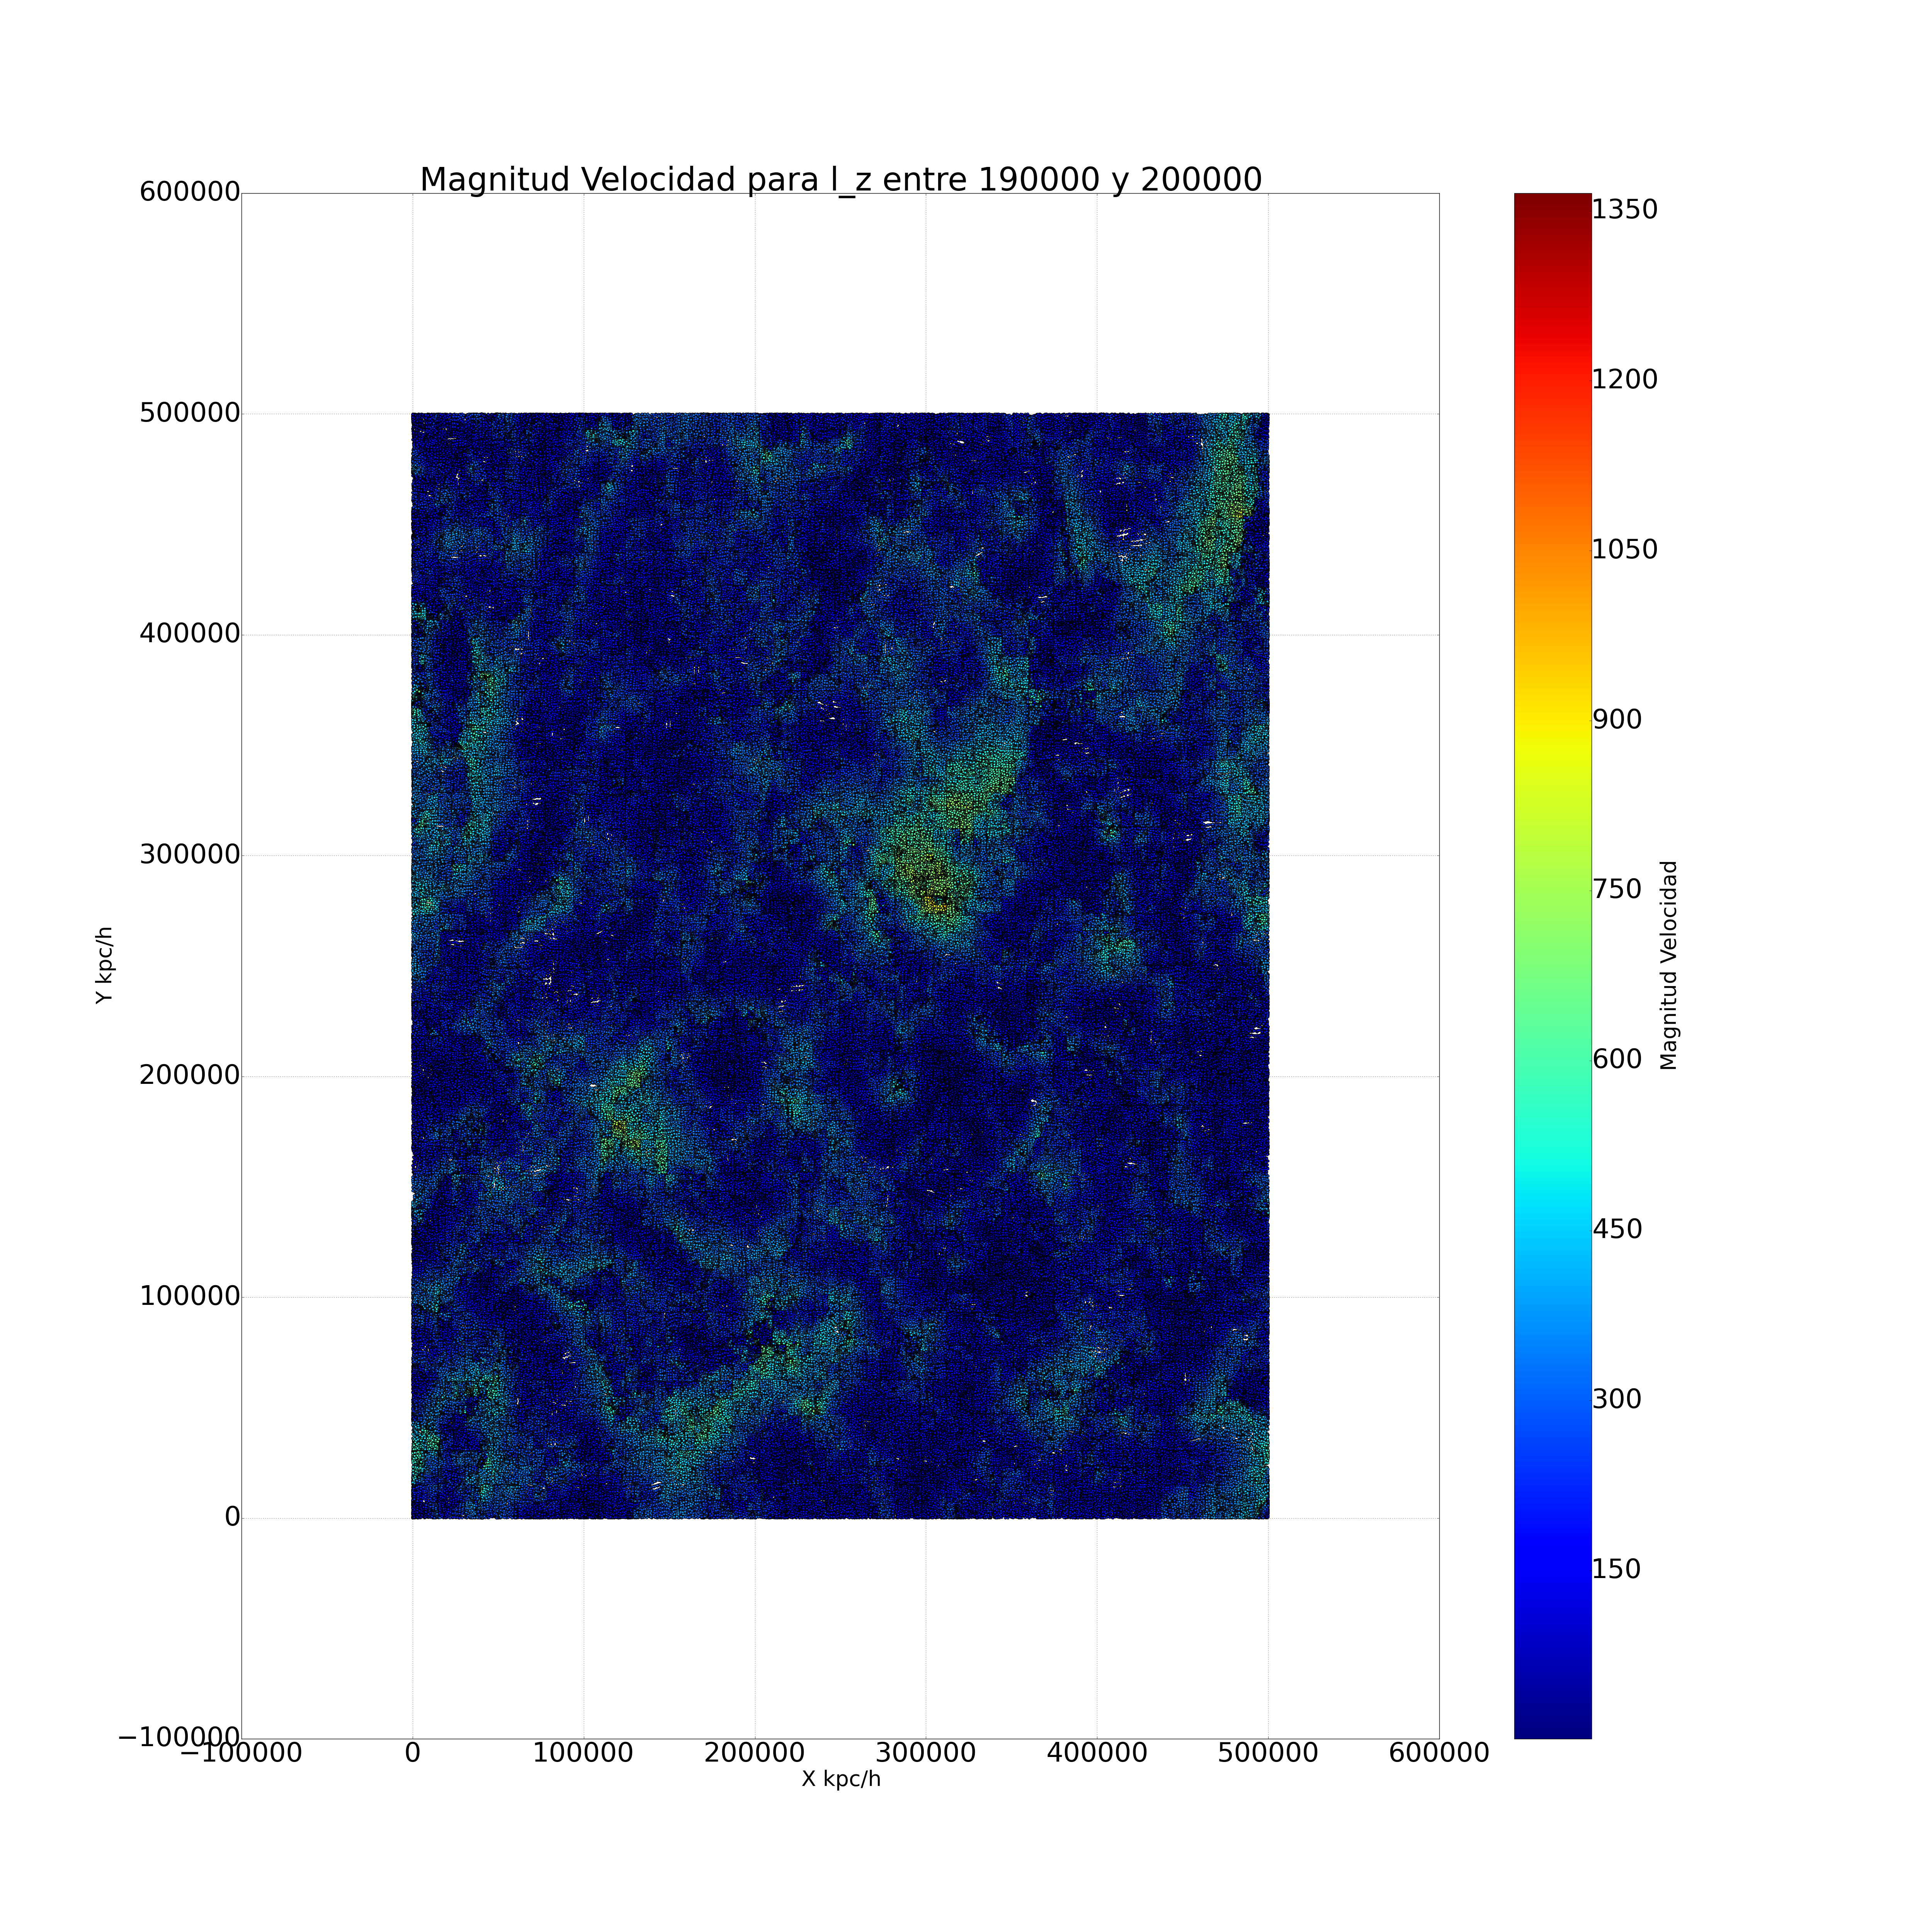
\includegraphics[width=0.9\textwidth]{graphs/scatter_magnitud_vel200000.png}
\end{minipage}
\caption{2D slices of the speed distribution}\label{fig:2D_slices}
\end{figure}
\FloatBarrier


We can observe in figure \ref{fig:2D_slices} intuitive signs of structures related to the speed distribution. 
We can observe filament structures\\

It is more clear if we observe from one side the particles with speed greater than a $th_{high}$ and the particles with speed lesser than a $th_{low}$.\\

\begin{figure}[ht]
\centering
\begin{minipage}{.45\textwidth}
  \centering
  \includegraphics[width=0.9\textwidth]{graphs/scatter_magnitud_vel_488_lz_100000.png}
\end{minipage}%
\begin{minipage}{.45\textwidth}
  \centering
  \includegraphics[width=0.9\textwidth]{graphs/scatter_magnitud_vel_488_lz_200000.png}
\end{minipage}
\begin{minipage}{.45\textwidth}
  \centering
  \includegraphics[width=0.9\textwidth]{graphs/scatter_magnitud_vel_59_lz_100000.png}
\end{minipage}
\begin{minipage}{.45\textwidth}
  \centering
  \includegraphics[width=0.9\textwidth]{graphs/scatter_magnitud_vel_59_lz_200000.png}
\end{minipage}
\caption{2D slices of the speed distribution. The upper slices with $|\vec{v}| > th_{high} = 488$ and the two lower slices with $|\vec{v}| < th_{low} = 59$ for the same cuts, $z = \{100, 200 \} Mpc/h$  }\label{fig:2D_slices_thresh}
\end{figure}
\FloatBarrier

As we can see in figure \ref{fig:2D_slices_thresh} the cuts with low and high thresholds are complementary. It is evident that structures are present. 

Finally we apply our region growing algorithm and we obtain the following results.\\

%Plot of the region identified.
\begin{figure}[ht]
\begin{center}
\includegraphics[width=0.8\textwidth]{graphs/regions_small.png} % Include the image placeholder.png
\caption{Region identified by the algorithm}
\label{fg:regions_speed_th_1}
\end{center}
\end{figure}
\FloatBarrier

And, changing the thresholds to: 
$th_{low} = \bar{v} + 2  \sigma_{v} = 488.48$ and $th_{high} = \bar{v}  +  8 \sigma_{v} =1195.0 $\\
We obtain:
%Plot of the region identified.
\begin{figure}[ht]
\begin{center}
\includegraphics[width=0.8\textwidth]{graphs/regions_big.png} % Include the image placeholder.png
\caption{Region identified by the algorithm with the second thresholds}
\label{fg:regions_speed_th_2}
\end{center}
\end{figure}
\FloatBarrier

We have different observations:\\
\begin{enumerate}
	\item The details of the regions in figures \ref{fg:regions_speed_th_1} and \ref{fg:regions_speed_th_2} seem accurate with what we would expect. It is more dense in the center and less dense in the borders.
	\item The regions obtained have a dimension of only a few Mpc/h (Laniakea's dimension is two orders of magnitude higher). This could mean that Laniakea is atypical. 
    \item There is first only one region identified. This indicates than all the high velocity particles are congregated in only one region (the detected region). If we set lower $th_{high}$ we can see we get more regions. 
    \item This is certainly a good naive approach to the problem. Nevertheless for more accurate results it needs to be drastically changed.
\end{enumerate}

The script in Appendix \ref{App:App_speed_code} was executed in a student's
laptop and later on the HPC cluster. For a significant number of particles, the laptop limited memory (8GB) crashes. Running in the HPC solves this issue. results.


\subsection{Code example for Region Growing Algorithm - Approach by the Speed} \label{App:App_speed_code}
\tiny
\lstinputlisting[language=Python, caption=Region Growing Algorithm Code]{code/region_detection_document.py}
\end{document} 

\section{Region Growing Algorithm with the FA and $tr\left(\sum_{\alpha\beta}\right)$} \label{App:own_impl_code}
\tiny
%TODO insert the code
Here comes the code.